\begin{adjustwidth*}{}{-2.25in}
\textbf{{\large Exercises}}
\setlength{\columnsep}{25pt}
\begin{multicols*}{2}
\noindent Terms and Concepts \small
\begin{enumerate}[1)]
\item T/F: Given a differentiable function $y=f(x)$, we are generally free to choose a value for $dx$, which then determines the value of $dy$.
\item T/F: The symbols ``$dx$'' and ``$\dx$'' represent the same concept.
\item T/F: The symbols ``$dy$'' and ``$\dy$'' represent the same concept.
\item T/F: Differentials are important in the study of integration.
\item When could the linearization of a function $f(x)$ at $x=a$ be a constant function?
\item How are differentials and tangent lines related?
\end{enumerate} 

\noindent {\normalsize Problems} \small

\noindent{\bf In exercises 7--11, use differentials to approximate the given value by hand.}

\begin{enumerate}[1),resume]
\item $2.05^2$
\item $5.1^3$
\item $\sqrt{16.5}$
\item $\sqrt[3]{63}$
\item $\sin 3$

\item A certain function $y=p(x)$ has its local linearization at $a = 3$ given by $L(x) = -2x + 5$.

\ba
	\item What are the values of $p(3)$ and $p'(3)$?  Why?
	\item Estimate the value of $p(2.79)$.
	\item Suppose that $p''(3) = 0$ and you know that $p''(x) < 0$ for $x < 3$.  Is your estimate in (b) too large or too small?
	\item Suppose that $p''(x) > 0$ for $x > 3$.  Use this fact and the additional information above to sketch an accurate graph of $y = p(x)$ near $x = 3$.  Include a sketch of $y = L(x)$ in your work.
\ea

%ITEM
\item A potato is placed in an oven, and the potato's temperature $F$ (in degrees Fahrenheit) at various points in time is taken and recorded in the following table. Time $t$ is measured in minutes.

\scalebox{.9}{
\begin{tabular}{|c||c|c|c|c|c|c|c|}
\hline
$t$ & $0$ & $15$ & $30$ & $45$ & $60$ & $75$ & $90$ \\ \hline% $F(t)$ \\ \hline \hline
$F(t)$ & $70$ & $180.5$ & $251$ & $296$ & $324.5$ & $342.8$ & $354.5$ \\ \hline
\end{tabular}
} % end scalebox

%\begin{tabular}{| l || l |}
%\hline
%$t$ & $F(t)$ \\ \hline \hline
%0 & 70\\ \hline
%15 & 180.5 \\ \hline
%30 & 251 \\ \hline
%45 & 296 \\ \hline
%60 & 324.5 \\ \hline
%75 & 342.8 \\ \hline
%90 & 354.5  \\ \hline
%\end{tabular}

\ba
	\item Use a central difference to estimate $F'(60)$.  Use this estimate as needed in subsequent questions.
	\item Find the local linearization $y = L(t)$ to the function $y = F(t)$ at the point where $a = 60$.
	\item Determine an estimate for $F(63)$ by employing the local linearization.  
	\item Do you think your estimate in (c) is too large or too small?  Why?
\ea

%ITEM
\item An object moving along a straight line path has a differentiable position function $y = s(t)$.  It is known that at time $t = 9$ seconds, the object's position is $s = 4$ feet (measured from its starting point at $t = 0$).  Furthermore, the object's instantaneous velocity at $t = 9$ is $-1.2$ feet per second, and its acceleration at the same instant is $0.08$ feet per second per second.

\ba
	\item Use local linearity to estimate the position of the object at $t = 9.34$.
	\item Is your estimate likely too large or too small?  Why?
	\item In everyday language, describe the behavior of the moving object at $t = 9$.  Is it moving toward its starting point or away from it? Is its velocity increasing or decreasing?
\ea

%ITEM
\item For a certain function $f$, its derivative is known to be $f'(x) = (x-1)e^{-x^2}$.  Note that you do not know a formula for $y = f(x)$.
\ba  
  	\item At what $x$-value(s) is $f'(x) = 0$?  Justify your answer algebraically, but include a graph of $f'$ to support your conclusion.
	\item Reasoning graphically, for what intervals of $x$-values is $f''(x) > 0$?  What does this tell you about the  behavior of the original function $f$?  Explain.
	\item Assuming that $f(2) = -3$, estimate the value of $f(1.88)$ by finding and using the tangent line approximation to $f$ at $x=2$.  Is your estimate larger or smaller than the true value of $f(1.88)$?  Justify your answer.
\ea
\end{enumerate}

\noindent{\bf In exercises 16--25, compute the differential.}

\begin{enumerate}[1),resume]
\item $y=x^2+3x-5$
\item $y=x^7-x^5$
\item $\ds y=\frac{1}{4x^2}$
\item $\ds y=(2x+\sin x)^2$
\item $\ds y=x^2e^{3x}$
\item $\ds y=\frac{4}{x^4}$
\item $\ds y=\frac{2x}{\tan x + 1}$
\item $\ds y=\ln (5x)$
\item $\ds y=e^x\sin x$
\item $\ds y=\cos (\sin x)$
\end{enumerate}

%------------------------------------------
% END OF EXERCISES ON FIRST PAGE
%------------------------------------------
\end{multicols*}
\end{adjustwidth*}

\clearpage

\begin{adjustwidth*}{}{-2.25in}
\setlength{\columnsep}{25pt}
\begin{multicols*}{2}\small

\begin{enumerate}[1),start=26]
\item A set of plastic spheres are to be made with a diameter of 1cm. If the manufacturing process is accurate to 1mm, what is the propagated error in volume of the spheres?

\item The distance, in feet, a stone drops in $t$ seconds is given by $d(t) = 16t^2$. The depth of a hole is to be approximated by dropping a rock and listening for it to hit the bottom. What is the propagated error if the time measurement is accurate to $2/10^{\text{ths}}$ of a second and the measured time is:
	\ba
	\item 2 seconds?
	\item	5 seconds?
	\ea

\item What is the propagated error in the measurement of the cross sectional area of a circular log if the diameter is measured at $15''$, accurate to $1/4''$?

\item A wall is to be painted that is $8'$ high and is measured to be $10',\ 7''$ long. Find the propagated error in the measurement of the wall's surface area if the measurement is accurate to $1/2''$. 

\item \label{exer:04_04_ex_34}The length $l$ of a long wall is to be calculated by measuring the angle $\theta$ shown in the diagram (not to scale). Assume the formed triangle is an isosceles triangle. The measured angle is $143^\circ$, accurate to $1^\circ$. 

\begin{minipage}{\linewidth}
\centering
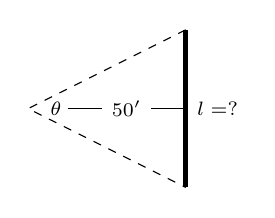
\begin{tikzpicture}
\draw [ultra thick] (1,-1) -- node [pos=.5,right] {\scriptsize $l=$?}(1,1);
\draw [dashed] (1,1) -- (-1,0) node [xshift=10pt] {\scriptsize $\theta$} -- (1,-1);
\draw (-.5,0) -- node [pos=.5,draw=white,fill=white] {\scriptsize $50'$} (1,0);
\end{tikzpicture}
\end{minipage}

\begin{enumerate}
\item		What is the measured length of the wall?
\item		What is the propagated error? 
\item		What is the percent error?
%\item		What is a key assumption about the location where the angle is measured? 
\end{enumerate}

\item \label{exer:04_04_ex_35} The length $l$ of a long wall is to be approximated. The angle $\theta$, as shown in the diagram (not to scale), is measured to be $85.2^\circ$, accurate to $1^\circ$. Assume that the triangle formed is a right triangle.

\begin{minipage}{\linewidth}
\centering
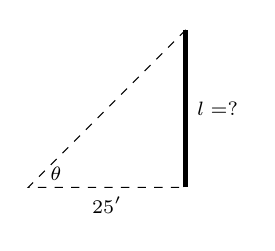
\begin{tikzpicture}
\draw [ultra thick] (1,-1) -- node [pos=.5,right] {\scriptsize $l=$?}(1,1);
\draw [dashed] (1,1) -- (-1,-1) node [xshift=10pt,yshift=5pt] {\scriptsize $\theta$} -- node [pos=.5,below] {\scriptsize $25'$} (1,-1);
%\draw (-.5,0) -- node [pos=.5,draw=white,fill=white] {\scriptsize $50'$} (1,0);
\end{tikzpicture}
\end{minipage}

\begin{enumerate}
\item		What is the measured length $l$ of the wall?
\item		What is the propagated error? 
\item		What is the percent error?
\end{enumerate}

\item \label{exer:04_04_ex_36} Answer the questions of Exercise \ref{exer:04_04_ex_35}, but with a measured angle of $71.5^\circ$, accurate to $1^\circ$, measured from a point $100'$ from the wall.

\item The length of the walls in Exercises \ref{exer:04_04_ex_35} -- \ref{exer:04_04_ex_34} are essentially the same. Which setup gives the most accurate result?

\item Consider the setup in Exercises \ref{exer:04_04_ex_34}. This time, assume the angle measurement of $143^\circ$ is exact but the measured $50'$ from the wall is accurate to $6''$. What is the approximate percent error?

%\item Use differentials to estimate the amount of paint needed to
%apply a coat of paint 0.02 cm thick to a sphere with diameter $40$
%meters. (Recall that the volume of a sphere of radius $r$ is $V
%=(4/3)\pi r^3$. Notice that you are given that $dr=0.02$.)
%%% \begin{answer} $dV=8\pi/25$

\end{enumerate}

\noindent{\bf Marginal Analysis.}

Differentials are used in economics to approximate changes in revenue, cost and profit. The  total revenue, $R$, for selling $x$ units of a product is given by
\[ R=xp\]  
When the number of units increases by one, the change in $x$ is $\delta x=1$, and the change in $R$ is \[ dR = \frac{dR}{dx} dx. \]
The differential $dR$ is the change in revenue that accompanies the sale of one additional unit and is called \emph{marginal revenue}. Similarly, differentials can be used to find the marginal profit, $dP$, and the marginal cost, $dC$. 
\begin{enumerate}[1),start=35]
\item		The demand function for a product is modeled by $p=\sqrt{400-x}$. What is the marginal revenue as sales increase from $256$ units to $257$ units?
\item		The profit derived from selling $x$ units of an item is modeled by $P=-0.5x^3+2500x-6000$. What is the marginal profit as sales increase from $50$ units to $51$ units?
\item		The cost of producing $x$ units of an item is modeled by $C=0.05x^2+4x+10$. What is the marginal cost as production increases from $12$ units to $13$ units?
\item 		Suppose the demand for a product is equal to the inverse of the square of the price. Find the marginal revenue when the price is $\$10$ per unit.
\end{enumerate}

%------------------------------------------------
% END OF EXERCISES ON SECOND PAGE
%------------------------------------------------
\end{multicols*}
\end{adjustwidth*}

\afterexercises